% 11/23/2015
%%%%%%%%%%%%%%%%%%%%%%%%%%%%%%%%%%%%%%%%%%%%%%%%%%%%%%%%%%%%%%%%%%%%%%%%%%%%
% AGUJournalTemplate.tex: this template file is for articles formatted with LaTeX
%
% This file includes commands and instructions
% given in the order necessary to produce a final output that will
% satisfy AGU requirements. 
%
% You may copy this file and give it your
% article name, and enter your text.
%
%%%%%%%%%%%%%%%%%%%%%%%%%%%%%%%%%%%%%%%%%%%%%%%%%%%%%%%%%%%%%%%%%%%%%%%%%%%%
% PLEASE DO NOT USE YOUR OWN MACROS
% DO NOT USE \newcommand, \renewcommand, or \def, etc.
%
% FOR FIGURES, DO NOT USE \psfrag or \subfigure.
% DO NOT USE \psfrag or \subfigure commands.
%%%%%%%%%%%%%%%%%%%%%%%%%%%%%%%%%%%%%%%%%%%%%%%%%%%%%%%%%%%%%%%%%%%%%%%%%%%%
%
% All questions should be e-mailed to latex@agu.org.
%
%%%%%%%%%%%%%%%%%%%%%%%%%%%%%%%%%%%%%%%%%%%%%%%%%%%%%%%%%%%%%%%%%%%%%%%%%%%%
%
% Step 1: Set the \documentclass
%
% There are two options for article format:
%
% 1) PLEASE USE THE DRAFT OPTION TO SUBMIT YOUR PAPERS.
% The draft option produces double spaced output.
% 
% 2) numberline will give you line numbers.

%% To submit your paper:
%\documentclass[draft,linenumbers]{agujournal}
%\draftfalse

%% For final version.
\documentclass{agujournal}
\usepackage{url}
% Now, type in the journal name: \journalname{<Journal Name>}

% ie, \journalname{Journal of Geophysical Research}
%% Choose from this list of Journals:
%
% JGR-Atmospheres
% JGR-Biogeosciences
% JGR-Earth Surface
% JGR-Oceans
% JGR-Planets
% JGR-Solid Earth
% JGR-Space Physics
% Global Biochemical Cycles
% Geophysical Research Letters
% Paleoceanography
% Radio Science
% Reviews of Geophysics
% Tectonics
% Space Weather
% Water Resource Research
% Geochemistry, Geophysics, Geosystems
% Journal of Advances in Modeling Earth Systems (JAMES)
% Earth's Future
% Earth and Space Science
%
%

\journalname{Journal of Advances in Modeling Earth Systems (JAMES)}


\begin{document}

%% ------------------------------------------------------------------------ %%
%  Title
% 
% (A title should be specific, informative, and brief. Use
% abbreviations only if they are defined in the abstract. Titles that
% start with general keywords then specific terms are optimized in
% searches)
%
%% ------------------------------------------------------------------------ %%

% Example: \title{This is a test title}

\title{A detailed total energy analysis of the Community Atmosphere Model (CAM)}

%% ------------------------------------------------------------------------ %%
%
%  AUTHORS AND AFFILIATIONS
%
%% ------------------------------------------------------------------------ %%

% Authors are individuals who have significantly contributed to the
% research and preparation of the article. Group authors are allowed, if
% each author in the group is separately identified in an appendix.)

% List authors by first name or initial followed by last name and
% separated by commas. Use \affil{} to number affiliations, and
% \thanks{} for author notes.  
% Additional author notes should be indicated with \thanks{} (for
% example, for current addresses). 

% Example: \authors{A. B. Author\affil{1}\thanks{Current address, Antartica}, B. C. Author\affil{2,3}, and D. E.
% Author\affil{3,4}\thanks{Also funded by Monsanto.}}

\authors{P.H. Lauritzen\affil{1}\thanks{1850 Table Mesa Drive, Boulder, Colorado, USA}, and D.L. Williamson \affil{1}}

 \affiliation{1}{National Center for Atmospheric Research, Boulder, Colorado, USA}
% \affiliation{2}{School of Marine and Atmospheric Sciences, Stony Brook University, State University of New York, Stony Brook, New York}
% \affiliation{3}{Sandia National Laboratories, Albuquerque, New Mexico, USA}
% \affiliation{4}{Department of Land, Air and Water Resources, University of California, Davis, California, USA}
% \affiliation{5}{Ecole Polytechnique, UMR 8539, Laboratoire de M\'et\'eorologie Dynamique/IPSL, Palaiseau, France}
% \affiliation{6}{Rosenstiel School of Marine and Atmospheric Science, University of Miami, Miami, Florida, USA}

% \affiliation{3}{Third Affiliation}
% \affiliation{4}{Fourth Affiliation}

%(repeat as many times as is necessary)

%% Corresponding Author:
% Corresponding author mailing address and e-mail address:

% (include name and email addresses of the corresponding author.  More
% than one corresponding author is allowed in this LaTeX file and for
% publication; but only one corresponding author is allowed in our
% editorial system.)  

% Example: \correspondingauthor{First and Last Name}{email@address.edu}

\correspondingauthor{Peter Hjort Lauritzen}{pel@ucar.edu}

%% Keypoints, final entry on title page.

% Example: 
% \begin{keypoints}
% \item	List up to three key points (at least one is required)
% \item	Key Points summarize the main points and conclusions of the article
% \item	Each must be 100 characters or less with no special characters or punctuation 
% \end{keypoints}

%  List up to three key points (at least one is required)
%  Key Points summarize the main points and conclusions of the article
%  Each must be 100 characters or less with no special characters or punctuation 

\begin{keypoints}
\item ...
%\item The CESM2.0 release of the spectral-element dynamical core (CAM-SE) is documented
%\item Model has comprehensive treatment of condensates and energy
%\item The CAM-SE model has been sped-up significantly compared to its predecessor CAM-HOMME
\end{keypoints}

%% ------------------------------------------------------------------------ %%
%
%  ABSTRACT
%
% A good abstract will begin with a short description of the problem
% being addressed, briefly describe the new data or analyses, then
% briefly states the main conclusion(s) and how they are supported and
% uncertainties. 
%% ------------------------------------------------------------------------ %%

%% \begin{abstract} starts the second page 

\begin{abstract}

\end{abstract}


%% ------------------------------------------------------------------------ %%
%
%  TEXT
%
%% ------------------------------------------------------------------------ %%

%%% Suggested section heads:
%\section{Introduction}
% 
% The main text should start with an introduction. Except for short
% manuscripts (such as comments and replies), the text should be divided
% into sections, each with its own heading. 

% Headings should be sentence fragments and do not begin with a
% lowercase letter or number. Examples of good headings are:

% \section{Materials and Methods}
% Here is text on Materials and Methods.
%
% \subsection{A descriptive heading about methods}
% More about Methods.
% 
% \section{Data} (Or section title might be a descriptive heading about data)
% 
% \section{Results} (Or section title might be a descriptive heading about the
% results)
% 
% \section{Conclusions}


\section{Introduction}
In coupled climate modeling with prognostic atmosphere, ocean, land, land-ice, and sea-ice components, it is important to conserve total energy to a high degree to avoid spurious long term trends in the simulated Earth system. Conservation of total energy in this context refers to having a closed total energy budget. For example, the total energy change in a column in the atmosphere is exactly balanced by the net sources/sinks given by the fluxes through the column. The fluxes into the atmospheric component from the surface models must be balanced by the fluxes in the respective surface components and so on. Henceforth we will focus only on the atmospheric component which, in a numerical model, is split into a resolved-scale component (the dynamical core) and a sub-grid-scale component (parameterizations or, in modeling jargon, physics). 

The atmospheric equations of motion conserve total energy but the discretizations used in climate and weather models are usually not inherently total energy conservative. Exact conservation is probably not necessary but conservation to within $~$0.01  $W/m^2$ has been considered sufficient to avoid spurious trends in century long simulations \citep{B2000S,WOHTTV2015JAMES}. Spurious sources and sinks of total energy can be introduced by the dynamical core, physics, physics-dynamics coupling as well as discrepancies between the total energy of the continuous and discrete equations of motion and for the physics. Hence the study of total energy conservation in comprehensive models of the atmosphere quickly becomes a quite complex and detailed matter. In addition there can easily be compensating errors in the system as a whole.

Here we focus on versions of the Community Atmosphere Model (CAM) that use the spectral-element \citep[SE, ][]{LetAl2018JAMES} and finite-volume \citep[FV, ][]{L2004MWR} dynamical cores. These dynamical cores couple with physics in a time-split manner, i.e. physics receives a state updated by dynamics \citep[see ][ for a discussion of time-split versus process split physics-dynamics coupling in the context of CAM]{W2002MWR}.

In its pure time-split form the physics tendencies are added to the state previously produced by the dynamical core and the resulting state provides the initial state for the subsequent dynamical core calculation. We refer to this as state-updating. Alternatively, when the dynamical core adopts a shorter time step than the physics, say N sub-steps, then (1/N)th of the physics-calculated tendency is added to the state before each dynamics sub-step. We refer to this modification of time-splitting as {\em{dribbling}}. CAM-FV uses the state-update approach while CAM-SE has options to use state-update, {\em{dribbling}} or a combination of the two (i.e. some variables use state-updating and others use {\em{dribbling}}). The dribbling variants can lead to spurious sources or sinks of total energy referred to as physics-dynamics coupling errors.

The dynamical core usually has implicit or explicit filters to control spurious noise near the grid scale which will lead to energy dissipation \citep{T2008JCP,JW2010LNCSE}. Similarly models often have sponge layers to control the solution near the top of the model that may be a sink of total energy. There are examples of numerical discretizations of the adiabatic frictionless equations motion that are designed so that total energy is conserved in the absence of time-truncation and filtering errors, e.g., mimetic spectral-element discretizations such as the one used in the horizontal in CAM-SE \citep{T2011LNCSEb}. These provide consistency between the discrete momentum and thermodynamic equations leading to global conservation associated with the conversion of potential to kinetic energy. In spectral transform models it is customary to add the energy change due to explicit diffusion on momentum back as heating (referred to as frictional heating), so that the diffusion of momentum does not affect the total energy budget \citep[see, e.g., p.71 in ][]{CAM5}. This is also done in CAM-SE \citep{LetAl2018JAMES}. 

It is the purpose of this paper to provide a detailed total energy analysis of the CAM-SE and CAM-FV. ...


%For example, the discrete total energy consistent with the dynamical core may differ from the one used in physics or,  even worse, the total energy that the continuous equations of motion conserve is different between the dynamical core and physics.\\

\section{Method}
\subsection{Defining total energy}
In the following it is assumed that the model top and bottom are coordinate surfaces and that there is no flux of mass through the model top and bottom. In a dry atmosphere the total energy equation integrated over the entire sphere is given by
\begin{equation}
\frac{d}{dt}\int_{z=z_s}^{z=z_{top}}\iint_{\Omega} E_v \rho^{(d)}\, dA\, dz=\int_{z=z_s}^{z=z_{top}}\iint_{\Omega} F_{net}\, \rho^{(d)} dA\, dz,
\end{equation}
\citep[e.g., ][]{K1974MWR} where $F_{net}$ is net fluxes calculated by the parameterizations (e.g., heating and momentum forcing), $d/dt$ the total/material derivative, $z_s$ is the height of the surface, $\Omega$ the sphere, $\rho^{(d)}$ the density of dry air and $E_v$ is the total energy. $E_v$ can be split into kinetic energy $K=\frac{1}{2}\vec{v}^2$ ($\mathbf{v}$ is the wind vector), internal energy $c_v^{(d)}T$, where $c_v^{(d)}$ is the heat capacity of dry air at constant volume, and potential energy $\Phi=gz$
\begin{equation}
E_v=K+c_v^{(d)}T+\Phi.
\end{equation}
If the vertical integral is performed in a mass-based vertical coordinate, e.g., pressure, then the integrated total energy equation for a dry atmosphere can be written as
\begin{equation}
\frac{d}{dt}\int_{p=p_s}^{p=p_{top}}\iint_{\Omega} E_p \rho^{(d)}\, dA\, dp + \frac{d}{dt}\iint_{\Omega}\Phi_sp_s dA =\int_{p=p_s}^{p=p_{top}}\iint_{\Omega} F_{net}\, \rho dA\, dp,
\end{equation}
\citep[e.g., ][]{K1974MWR} where
\begin{equation}
E_p=K+c_p^{(d)}T.
\end{equation}
In a moist atmosphere, however, there are several definitions of total energy used in the literature related to what heat capacity is used for water vapor and whether or not condensates are accounted for in the energy equation. To explain the details of that we focus on the energy equation for CAM-SE.

CAM-SE is formulated using a terrain-following hybrid-sigma vertical coordinate $\eta$ but the coordinate levels are defined in terms of dry air mass ($M^{(d)}$) instead of total air mass; $\eta^{(d)}$ \citep[see ][ for details]{LetAl2018JAMES}. In such a coordinate system it is convenient to define the tracer state in terms of a dry mixing ratio instead of moist mixing ratio
\begin{equation}
m^{(\ell)}\equiv \frac{\rho^{(\ell)}}{\rho^{(d)}}, \text{ where }\ell=`wv`,`cl`,`ci`,`rn`,`sw`,\label{eq:mx}
\end{equation}
where $\rho^{(d)}$ is the mass of dry air per unit volume of moist air and $\rho^{(\ell)}$ is the mass of the water substance of type $\ell$ per unit volume of moist air. Moist air refers to air containing dry air (`d`), water vapor (`wv`), cloud liquid (`cl`), cloud ice (`ci`), rain amount(`rn`) and snow amount(`sw`). For notational purposes define the set of all components of air
\begin{equation}
\mathcal{L}_{all}=\left\{ `d`,`wv`,`cl`,`ci`,`rn`,`sw`\right\},
\end{equation}
Define associated heat capacities at constant pressure $c_p^{(\ell)}$. Using the $\eta^{(d)}$ vertical coordinate and dry mixing ratios the total energy that the frictionless adiabatic equations of motion in the CAM-SE dynamical core conserves is 
\begin{equation}
\left< E^{(dycore)}\right>=\int_{\eta=0}^{\eta=1} \iint_\mathcal{S} \left( \frac{\partial M^{(d)}}{\partial \eta^{(d)}} \right)\sum_{\ell \in \mathcal{L}_{all}} \left[m^{(\ell)} \left(K+c_p^{(\ell)}T+\Phi_s  \right)\right]  dA d \eta^{(d)},\label{eq:comprehensice_energy}
\end{equation}
where $\Phi_s$ is the surface geopotential.

In the CAM physical parameterizations a different definition of total energy is used. Due to the evolutionary nature of the model development, the parameterizations have not yet been converted to match the SE dynamical core. For the computation of total energy condensates are assumed to be zero and the heat capacity of moisture is the same as for dry air. This is equivalent to using a moist mass (dry air plus water vapor) but $c_p$ of dry air.
\begin{equation}
\label{eq:Ephys}
\left< E^{(physics)}\right> =\int_{\eta=0}^{\eta=1} \iint_\mathcal{S} \left( \frac{\partial M^{(d)}}{\partial \eta^{(d)}} \right)\left(1+m^{(wv)}\right)\left[ \left(K+c_p^{(d)}T+\Phi_s\right)\right]dA d \eta^{(d)}.
\end{equation}
We note that earlier versions of CAM using the spectral transform dynamical core used $c_p$ of moist air. 
One can make the adiabatic, frictionless equations of motion in the dynamical core conserve $E^{(physics)}$ by not including condensates in the mass/pressure field as well as energy conversion term in the thermodynamic equation and setting the heat capacity for moisture to $c_p^{(d)}$ \citep{T2011LNCSEb}. We will also make use of this configuration in the analysis presented in this paper.


\subsection{Spurious energy sources and sinks}
In a weather/climate model total energy conservation errors can appear in many places throughout the algorithm. Below is a general list of where conservation errors can appear with specific examples from CAM:
\begin{itemize}
\item {\em{Parameterization errors}}: Individual parameterizations may not have a closed energy budget. However, CAM parameterizations are required to have a closed energy budget under the assumption that pressure remains constant during the computation of the subgrid-scale parameterization tendencies. In other words, the total energy change in the column is exactly balanced by the net sources/sinks given by the fluxes through the column. 
\item {\em{Pressure work}}: That said, if parameterizations update specific humidity then the surface pressure changes (e.g., moisture leaving the column). In that case the pressure changes which, in turn, changes total energy, here referred to as {\em{pressure work}} \citep[section 3.1.8 in ][]{CAM5}.
\item {\em{Physics-dynamics coupling (PDC)}}: Assume that physics computes a tendency. Usually the tendency is passed to the dynamical core which is responsible for adding the tendencies to the state before advancing the dynamics. PDC energy errors can be split into two types:
\begin{itemize}
\item {\em{`Dribbling' errors (or, equivalently, temporal PDC errors)}}: If the total energy increment from the parameterizations does not match the change in total energy when the tendencies are added to the state in the dynamical core, then there will be a spurious PDC error. This will not happen with the state-update approach in which the tendencies are added immediate after physics and before the dynamical core advances the solution in time, but it does happen with dribbling. 
\item {\em{Change of vertical grid/coordinate errors}}: If the vertical coordinate in physics and in the dynamical core are different then there can be spurious PDC energy errors even when using the state-update method for adding tendencies to the dynamical core state. For example, many non-hydrostatic dynamical cores \citep[e.g. MPAS, ]{MPASatm} use a terrain-following height coordinate whereas physics uses pressure.
\item {\em{Change of horizontal grid errors:}} If the physics tendencies are computed on a different horizontal grid than the dynamical core then there can be spurious energy errors from mapping tendencies between horizontal grids \citep[e.g., ][]{HetAl2018MWR}. 
\end{itemize}
\item {\em{Dynamical core errors}}: Energy conservation errors in the dynamical core, not related to PDC errors, can arise in multiple parts of the algorithms used to solve the equations of motion. For dynamical cores employing implicit filtering \citep[e.g., limiters in flux operators ][]{L2004MWR} and/or possessing inherent damping to control small scales, it is hard to diagnose what their energy dissipation is compared to other errors in the discretization. If explicit filtering is used, e.g., hyperviscosity on momentum, then one can diagnose the energy dissipation from filtering and add a corresponding heating to balance it. There may also be energy loss from viscosity applied to other variables such a temperature or surface pressure which are harder to compensate. Here is a beak-down relevant to CAM-SE using a floating Lagrangian vertical coordinate:
\begin{itemize}
\item Horizontal inviscid dynamics: Energy errors resulting from solving the inviscid, adiabatic equations of motion.
\item Hyperviscosity: Filtering errors.
\item Vertical remapping: The vertical remapping algorithm does not conserve total energy.
\item Near round-off negative values
\end{itemize}
\item {\em{Continuous total energy formula discrepancy}}:  If the continuous equations of motion for the dynamical core conserve a total energy different from the one used in the parameterizations then an energy inconsistency is present in the system as a whole. This is the case with the new version of CAM-SE that conserves a total energy that is more accurate and comprehensive than the CAM physics package as discussed above. As also noted above, this mismatch arose from the evolutionary nature of the model development and not by deliberate design.
\end{itemize}
To avoid total energy conservation errors which could accumulate and ultimately lead to a climate drift, it is customary to use an energy fixer to restore total energy conservation. Since the spatial distribution of energy errors, in general, is not known, global fixers are used. In CAM a uniform increment is added to the temperature field to compensate for total energy loss in the dynamical core, physics-dynamics coupling and energy change dues to pressure work. 
%
\section{Results}
\subsection{Temporal averaging}
 \begin{figure}[h]
 \centering
 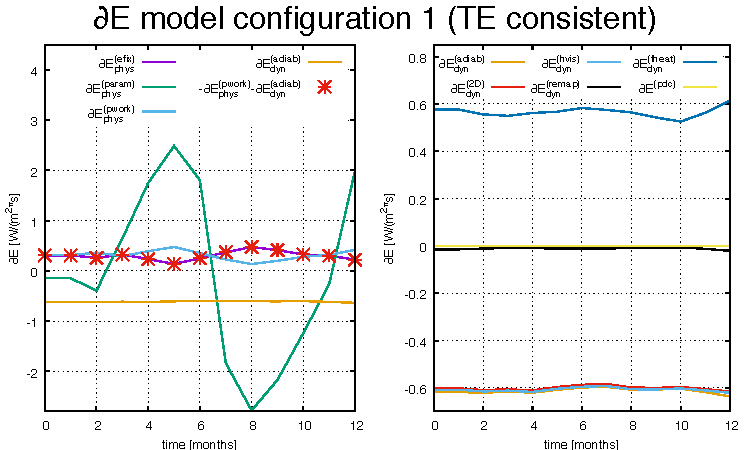
\includegraphics[width=35pc]{figs/dEdt.pdf}
 \caption{{\color{red}{[in note form] Note that the parameterizations have a closed energy budget so the fluctuations in the energy change due to parameterizations is balanced by fluxes in/out of the physics columns. The purpose of this Figure is to show that the energy tendency in the dynamical core is quite constant (to within ~0.2 $W/m^2$ or less); so only one month simulation may be enough to assess energy diagnostics for the dynamical core. DME adjust fluctuates with the physics forcing; obviously the energy fixers fluctuates with DME adjust. The {\em{consistency check}} (triangles) shows that the energy fixer exactly compensates for total energy loss in dynamical core and dme adjust (there are no physics dynamics coupling errors in this configuration).}}}
 \label{figone}
  \end{figure}


`The discrepancy between the more comprehensive energy formula \eqref{eq:comprehensice_energy} and the CAM physics formula for total energy is about 0.5 $W/m^2$ \citep{T2011LNCSEb}. By only including dry air and water vapor   in $\rho$ and setting $c_p^{(wv)}= c_p^{(d)}$ in the equations of motion, the dynamical core (in the absence of truncation errors) will conserve the energy used in CAM physics.'

\subsection{Configuration 1: Consistent total energy definitions in parameterizations and dynamical core, and total energy conserving physics-dynamics coupling}
This configuration is most energetically consistent in that the physical parameterizations and the continuous equations of motion on which the dynamical is based, conserve the same total energy $\left< E^{(physics)}\right>$ defined in equation \eqref{eq:Ephys}; and there are no spurious sources/sinks in physics-dynamics coupling. Energetic consistency in dynamics and physics is obtained by setting $c_p^{(\ell)}\equiv c_p^{d}\equiv$ and $\mathcal{L}_{all}=\left\{ `d`,`wv`\right\}$. If the parameterizations effectively update the model state then there are no physics-dynamics coupling errors \citep[$\tt{ftype=1}$ setup described in detail in ][]{LetAl2018JAMES}. Namelist changes resulting in this configuration are $\tt{lcp\_moist}=.true.$, $\tt{se\_qsize\_condensate\_loading=1}$, and $\tt{ftype=1}$.
\begin{figure}[h]
% \centering
% when using pdflatex, use pdf file:

\verb+do nt=1,ntotal+\\
\verb+  +\\
\verb+  PARAMETERIZATIONS:+\\
\verb+  +\\
\verb+  +{\color{blue}{output 'pBF'}}\\
\verb+  +Energy fixer\\
\verb+  +{\color{blue}{output 'pBP'}}\\
\verb+  +Physics updates the state and state saved for energy fixer\\
\verb+  +{\color{blue}{output 'pAP'}}\\
\verb+  +Dry mass correction\\
\verb+  +{\color{blue}{output 'pAM'}}\\
\verb+  +\\
\verb+  DYNAMICAL CORE:+\\
\verb+  +\\
\verb+  +{\color{blue}{output 'dED'}}\\
\verb+  do ns=1,nsplit+\\
\verb+    +{\color{blue}{output 'dAF'}}\\
\verb+    Update state with (1/nsplit) of the physics tendencies+\\
\verb+    +{\color{blue}{output 'dBD'}}\\
\verb+    do nr=1,rsplit+\\
\verb+       Advance the adiabatic frictionless equations of motion +\\
\verb+       in floating Lagrangian layer.+\\
\verb+       do ns=1,hypervis_subcycle+\\
\verb+          +{\color{blue}{output 'dBH'}}\\
\verb+          Advance hyperviscosity operators.+\\
\verb+          +{\color{blue}{output 'dCH'}}\\
\verb+          Add frictional heating to temperature.+\\
\verb+          +{\color{blue}{output 'dAH'}}\\
\verb+       end do+\\
\verb+    end do+\\
\verb+    +{\color{blue}{output 'dAD'}}\\
\verb+    Vertical remapping from floating Lagrangian levels to Eulerian levels+\\
\verb+    +{\color{blue}{output 'dAR'}}\\
\verb+  end do+\\
\verb+  +{\color{blue}{output 'dBF'}}\\
\verb+end do+
\caption{Pseudo-code ...}
\end{figure}

\section{Conclusions}\label{sec:concl}

%Text here ===>>>

%%
%  Numbered lines in equations:
%  To add line numbers to lines in equations,
%  \begin{linenomath*}
%  \begin{equation}
%  \end{equation}
%  \end{linenomath*}



%% Enter Figures and Tables near as possible to where they are first mentioned:
%
% DO NOT USE \psfrag or \subfigure commands.
%
% Figure captions go below the figure.
% Table titles go above tables;  other caption information
%  should be placed in last line of the table, using
% \multicolumn2l{$^a$ This is a table note.}
%
%----------------
% EXAMPLE FIGURE
%
% \begin{figure}[h]
% \centering
% when using pdflatex, use pdf file:
% \includegraphics[width=20pc]{figsamp.pdf}
%
% when using dvips, use .eps file:
% \includegraphics[width=20pc]{figsamp.eps}
%
% \caption{Short caption}
% \label{figone}
%  \end{figure}
%
% ---------------
% EXAMPLE TABLE
%
% \begin{table}
% \caption{Time of the Transition Between Phase 1 and Phase 2$^{a}$}
% \centering
% \begin{tabular}{l c}
% \hline
%  Run  & Time (min)  \\
% \hline
%   $l1$  & 260   \\
%   $l2$  & 300   \\
%   $l3$  & 340   \\
%   $h1$  & 270   \\
%   $h2$  & 250   \\
%   $h3$  & 380   \\
%   $r1$  & 370   \\
%   $r2$  & 390   \\
% \hline
% \multicolumn{2}{l}{$^{a}$Footnote text here.}
% \end{tabular}
% \end{table}

%% SIDEWAYS FIGURE and TABLE 
% AGU prefers the use of {sidewaystable} over {landscapetable} as it causes fewer problems.
%
% \begin{sidewaysfigure}
% \includegraphics[width=20pc]{figsamp}
% \caption{caption here}
% \label{newfig}
% \end{sidewaysfigure}
% 
%  \begin{sidewaystable}
%  \caption{Caption here}
% \label{tab:signif_gap_clos}
%  \begin{tabular}{ccc}
% one&two&three\\
% four&five&six
%  \end{tabular}
%  \end{sidewaystable}

%% If using numbered lines, please surround equations with \begin{linenomath*}...\end{linenomath*}
%\begin{linenomath*}
%\begin{equation}
%y|{f} \sim g(m, \sigma),
%\end{equation}
%\end{linenomath*}

%%% End of body of article

%%%%%%%%%%%%%%%%%%%%%%%%%%%%%%%%
%% Optional Appendix goes here
%
% The \appendix command resets counters and redefines section heads
%
% After typing \appendix
%
%\section{Here Is Appendix Title}
% will show
% A: Here Is Appendix Title
%
\appendix
   \section{...}

%\section{Here is a sample appendix}

%%%%%%%%%%%%%%%%%%%%%%%%%%%%%%%%%%%%%%%%%%%%%%%%%%%%%%%%%%%%%%%%
%
% Optional Glossary, Notation or Acronym section goes here:
%
%%%%%%%%%%%%%%  
% Glossary is only allowed in Reviews of Geophysics
%  \begin{glossary}
%  \term{Term}
%   Term Definition here
%  \term{Term}
%   Term Definition here
%  \term{Term}
%   Term Definition here
%  \end{glossary}

%
%%%%%%%%%%%%%%
% Acronyms
%   \begin{acronyms}
%   \acro{Acronym}
%   Definition here
%   \acro{EMOS}
%   Ensemble model output statistics 
%   \acro{ECMWF}
%   Centre for Medium-Range Weather Forecasts
%   \end{acronyms}

%
%%%%%%%%%%%%%%
% Notation 
%   \begin{notation}
%   \notation{$a+b$} Notation Definition here
%   \notation{$e=mc^2$} 
%   Equation in German-born physicist Albert Einstein's theory of special
%  relativity that showed that the increased relativistic mass ($m$) of a
%  body comes from the energy of motion of the body—that is, its kinetic
%  energy ($E$)—divided by the speed of light squared ($c^2$).
%   \end{notation}




%%%%%%%%%%%%%%%%%%%%%%%%%%%%%%%%%%%%%%%%%%%%%%%%%%%%%%%%%%%%%%%%
%
%  ACKNOWLEDGMENTS
%
% The acknowledgments must list:
%
% •	All funding sources related to this work from all authors
%
% •	Any real or perceived financial conflicts of interests for any
%	author
%
% •	Other affiliations for any author that may be perceived as
% 	having a conflict of interest with respect to the results of this
% 	paper.
%
% •	A statement that indicates to the reader where the data
% 	supporting the conclusions can be obtained (for example, in the
% 	references, tables, supporting information, and other databases).
%
% It is also the appropriate place to thank colleagues and other contributors. 
% AGU does not normally allow dedications.


\acknowledgments
The National Center for Atmospheric Research is sponsored by the National Science Foundation. We thank NCAR's Computational and Information Systems Laboratory (CISL) and NCAR's Climate and Global Dynamics division (CGD) for computational resources.

%We thank two anonymous reviewers for their helpful comments and time put into reviewing this very long/technical paper. Herrington, Reed and Lauritzen are grateful to the NCAR Advance Study Program graduate visitor program for funding Herrington's 9-month visit to NCAR. We thank NCAR's Computational and Information Systems Lab (CISL) for providing computing support. Goldhaber was partially supported by the U.S. Department of Energy Office of Biological and Environmental Research, Work Package 12-015334 ``Multiscale Methods for Accurate, Efficient, and Scale-Aware Models of the Earth System''. Medeiros acknowledges support by the Regional and Global Climate Modeling Program of the U.S. Department of Energy's Office of Science,  Cooperative Agreement DE-FC02-97ER62402. Benedict was funded by National Science Foundation (NSF) Rapid Response Research (RAPID) award AGS-1547910. The data presented in this manuscript is available at {\url{https://github.com/PeterHjortLauritzen/2017-JAMES-CESM2-SE.git}}.

%% ------------------------------------------------------------------------ %%
%% Citations

% Please use ONLY \citet and \citep for reference citations.
% DO NOT use other cite commands (e.g., \cite, \citeyear, \nocite, \citealp, etc.).


%% Example \citet and \citep:
%  ...as shown by \citet{Boug10}, \citet{Buiz07}, \citet{Fra10},
%  \citet{Ghel00}, and \citet{Leit74}. 

%  ...as shown by \citep{Boug10}, \citep{Buiz07}, \citep{Fra10},
%  \citep{Ghel00, Leit74}. 

%  ...has been shown \citep [e.g.,][]{Boug10,Buiz07,Fra10}.



%%  REFERENCE LIST AND TEXT CITATIONS

\bibliography{bib}
%
% Either type in your references using
%
% \begin{thebibliography}{}
% \bibitem[{\textit{Kobayashi et~al.}}(2003)]{R2013} Kobayashi, T.,
% Tran, A.~H., Nishijo, H., Ono, T., and Matsumoto, G.  (2003).
% Contribution of hippocampal place cell activity to learning and
% formation of goal-directed navigation in rats. \textit{Neuroscience}
% 117, 1025--1035.
%
% \bibitem{}
% Text
% \end{thebibliography}
%
%\bibliography{bib}
%%%%%%%%%%%%%%%%%%%%%%%%%%%%%%%%%%%%%%%%%%%%%%%
% Or, to use BibTeX:
%
% Follow these steps
%
% 1. Type in \bibliography{<name of your .bib file>} 
%    Run LaTeX on your LaTeX file.
%
% 2. Run BiBTeX on your LaTeX file.
%
% 3. Open the new .bbl file containing the reference list and
%   copy all the contents into your LaTeX file here.
%
% 4. Run LaTeX on your new file which will produce the citations.
%
% AGU does not want a .bib or a .bbl file. Please copy in the contents of your .bbl file here.


%% After you run BibTeX, Copy in the contents of the .bbl file here:


%%%%%%%%%%%%%%%%%%%%%%%%%%%%%%%%%%%%%%%%%%%%%%%%%%%%%%%%%%%%%%%%%%%%%
% Track Changes:
% To add words, \added{<word added>}
% To delete words, \deleted{<word deleted>}
% To replace words, \replace{<word to be replaced>}{<replacement word>}
% To explain why change was made: \explain{<explanation>} This will put
% a comment into the right margin.

%%%%%%%%%%%%%%%%%%%%%%%%%%%%%%%%%%%%%%%%%%%%%%%%%%%%%%%%%%%%%%%%%%%%%
% At the end of the document, use \listofchanges, which will list the
% changes and the page and line number where the change was made.

% When final version, \listofchanges will not produce anything,
% \added{<word or words>} word will be printed, \deleted{<word or words} will take away the word,
% \replaced{<delete this word>}{<replace with this word>} will print only the replacement word.
%  In the final version, \explain will not print anything.
%%%%%%%%%%%%%%%%%%%%%%%%%%%%%%%%%%%%%%%%%%%%%%%%%%%%%%%%%%%%%%%%%%%%%

%%%
\listofchanges
%%%

\end{document}

%%%%%%%%%%%%%%%%%%%%%%%%%%%%%%%%%%%%%
%% Supporting Information
%% (Optional) See AGUSuppInfoSamp.tex/pdf for requirements 
%% for Supporting Information.
%%%%%%%%%%%%%%%%%%%%%%%%%%%%%%%%%%%%%



%%%%%%%%%%%%%%%%%%%%%%%%%%%%%%%%%%%%%%%%%%%%%%%%%%%%%%%%%%%%%%%

More Information and Advice:

%% ------------------------------------------------------------------------ %%
%
%  SECTION HEADS
%
%% ------------------------------------------------------------------------ %%

% Capitalize the first letter of each word (except for
% prepositions, conjunctions, and articles that are
% three or fewer letters).

% AGU follows standard outline style; therefore, there cannot be a section 1 without
% a section 2, or a section 2.3.1 without a section 2.3.2.
% Please make sure your section numbers are balanced.
% ---------------
% Level 1 head
%
% Use the \section{} command to identify level 1 heads;
% type the appropriate head wording between the curly
% brackets, as shown below.
%
%An example:
%\section{Level 1 Head: Introduction}
%
% ---------------
% Level 2 head
%
% Use the \subsection{} command to identify level 2 heads.
%An example:
%\subsection{Level 2 Head}
%
% ---------------
% Level 3 head
%
% Use the \subsubsection{} command to identify level 3 heads
%An example:
%\subsubsection{Level 3 Head}
%
%---------------
% Level 4 head
%
% Use the \subsubsubsection{} command to identify level 3 heads
% An example:
%\subsubsubsection{Level 4 Head} An example.
%
%% ------------------------------------------------------------------------ %%
%
%  IN-TEXT LISTS
%
%% ------------------------------------------------------------------------ %%
%
% Do not use bulleted lists; enumerated lists are okay.
% \begin{enumerate}
% \item
% \item
% \item
% \end{enumerate}
%
%% ------------------------------------------------------------------------ %%
%
%  EQUATIONS
%
%% ------------------------------------------------------------------------ %%

% Single-line equations are centered.
% Equation arrays will appear left-aligned.

Math coded inside display math mode \[ ...\]
 will not be numbered, e.g.,:
 \[ x^2=y^2 + z^2\]

 Math coded inside \begin{equation} and \end{equation} will
 be automatically numbered, e.g.,:
 \begin{equation}
 x^2=y^2 + z^2
 \end{equation}


% To create multiline equations, use the
% \begin{eqnarray} and \end{eqnarray} environment
% as demonstrated below.
\begin{eqnarray}
  x_{1} & = & (x - x_{0}) \cos \Theta \nonumber \\
        && + (y - y_{0}) \sin \Theta  \nonumber \\
  y_{1} & = & -(x - x_{0}) \sin \Theta \nonumber \\
        && + (y - y_{0}) \cos \Theta.
\end{eqnarray}

%If you don't want an equation number, use the star form:
%\begin{eqnarray*}...\end{eqnarray*}

% Break each line at a sign of operation
% (+, -, etc.) if possible, with the sign of operation
% on the new line.

% Indent second and subsequent lines to align with
% the first character following the equal sign on the
% first line.

% Use an \hspace{} command to insert horizontal space
% into your equation if necessary. Place an appropriate
% unit of measure between the curly braces, e.g.
% \hspace{1in}; you may have to experiment to achieve
% the correct amount of space.


%% ------------------------------------------------------------------------ %%
%
%  EQUATION NUMBERING: COUNTER
%
%% ------------------------------------------------------------------------ %%

% You may change equation numbering by resetting
% the equation counter or by explicitly numbering
% an equation.

% To explicitly number an equation, type \eqnum{}
% (with the desired number between the brackets)
% after the \begin{equation} or \begin{eqnarray}
% command.  The \eqnum{} command will affect only
% the equation it appears with; LaTeX will number
% any equations appearing later in the manuscript
% according to the equation counter.
%

% If you have a multiline equation that needs only
% one equation number, use a \nonumber command in
% front of the double backslashes (\\) as shown in
% the multiline equation above.

% If you are using line numbers, remember to surround
% equations with \begin{linenomath*}...\end{linenomath*}

%  To add line numbers to lines in equations:
%  \begin{linenomath*}
%  \begin{equation}
%  \end{equation}
%  \end{linenomath*}



